\documentclass{article}
\usepackage[utf8]{inputenc}
\usepackage{geometry}
\geometry{a4paper, margin=1in}
\usepackage{hyperref}
\usepackage{graphicx}

\title{GigTim --- Product Brief \& Requirements Specification}
\author{Design Brief}
\date{\today}

\begin{document}

\maketitle

\section{Product Concept \& Market Context}
\textbf{GigTim} is a local gig-economy marketplace connecting temporary day-laborers (\textit{zilieri}) with hospitality (HoReCa) and local service businesses in Romania. 

Unlike general freelancer marketplaces, GigTim focuses on:
\begin{itemize}
    \item \textbf{Immediate shift-based work}: Simple, short-term shifts (e.g., a waiter needed for 8 hours at an event, a barista for a weekend peak, or a dishwasher for a day).
    \item \textbf{Legal compliance}: Under Romanian day-labor law, employers must submit worker registration sheets to the ITM (\textit{Inspectoratul Teritorial de Muncă}). The platform facilitates the gathering of compliant details (Romanian CNP and CI card series) to support this.
    \item \textbf{Reputation \& reliability}: A strong rating and review system to ensure workers show up and businesses maintain safe, professional working environments.
\end{itemize}

\section{Target User Personas \& Goals}

\subsection{The Worker (Zilier)}
\begin{itemize}
    \item \textbf{Who they are}: Individuals looking for flexible, quick-paying jobs, students, or hospitality professionals wanting to fill open days.
    \item \textbf{Core Goals}:
    \begin{itemize}
        \item Browse and apply to shifts matching their role, location, and desired hourly rate.
        \item Coordinate details with employers directly.
        \item Track scheduled shifts and maintain a high reliability rating.
        \item Quickly register, complete profile verification, and upload compliance data.
    \end{itemize}
\end{itemize}

\subsection{The Employer (Business)}
\begin{itemize}
    \item \textbf{Who they are}: Restaurant owners, event organizers, café managers, or warehouse managers needing quick temporary staff.
    \item \textbf{Core Goals}:
    \begin{itemize}
        \item Post open shifts with dates, duration, role descriptions, and hourly pay.
        \item Review applications and select qualified candidates based on experience and ratings.
        \item Start quick chat sessions with applicants to ask screening questions.
        \item Accept workers and export their registration information to submit for local labor compliance (ITM).
        \item Rate workers after the shifts are completed.
    \end{itemize}
\end{itemize}

\section{Core Features \& Functional Requirements}

\subsection{Authentication \& Role Selection}
\begin{itemize}
    \item \textbf{Sign Up / Sign In}: Email/password authentication.
    \item \textbf{Role Distinction}: Users must register as either a \texttt{WORKER} or an \texttt{EMPLOYER}.
    \item \textbf{Registration Fields}:
    \begin{itemize}
        \item \textbf{Workers}: Name, phone, city, CNP (13-digit Romanian personal identification number), and CI series/number (National ID).
        \item \textbf{Employers}: Company name, CUI (Romanian unique fiscal registration code), company headquarters address, and city.
    \end{itemize}
\end{itemize}

\subsection{Jobs Marketplace}
\begin{itemize}
    \item \textbf{Browse open shifts}: A feed showing active job listings.
    \item \textbf{Search \& Filters}: Users need to filter by city location, job roles (e.g. Barista, Waiter, Dishwasher, Stagehand), and sort by date or pay rate.
    \item \textbf{Job Posting Details}: Displays company name, hourly pay in RON, shift duration, role category, start/end times, city location, and total estimated payout.
    \item \textbf{Apply Action}: Workers can apply to open shifts. Once applied, the option locks to prevent duplicate applications.
\end{itemize}

\subsection{Messaging \& Connection Hub}
\begin{itemize}
    \item \textbf{Employer-Worker Chat}: A messaging center enabling communication to coordinate shift logistics.
    \item \textbf{Chat Access Points}:
    \begin{itemize}
        \item Employers can initiate a chat directly from a candidate's application card.
        \item Workers can message an employer directly from a job posting details screen.
        \item A directory of potential connections (employers see workers, workers see employers) is available to start discussions.
    \end{itemize}
\end{itemize}

\subsection{Shift \& Application Tracker}
\begin{itemize}
    \item \textbf{Employers}:
    \begin{itemize}
        \item Monitor active, upcoming, and past shifts.
        \item View lists of candidates split by status: ``În așteptare'' (Pending evaluation) and ``Procesate'' (Accepted or Rejected).
        \item Accept or reject candidates.
        \item \textbf{ITM CSV Export}: Accepting a worker generates an easy CSV download containing the worker's full name, CNP, and CI details for legal labor reporting.
    \end{itemize}
    \item \textbf{Workers}:
    \begin{itemize}
        \item Track upcoming confirmed shifts they are scheduled to work.
        \item View application status logs.
    \end{itemize}
\end{itemize}

\subsection{Profile \& Reputation System}
\begin{itemize}
    \item \textbf{Reputation Metrics}: Display of reliability ratings, total completed shifts, and lists of past feedback reviews.
    \item \textbf{Zero Review State}: New users with 0 reviews need to display clean placeholder states (e.g., ``0 recenzii'') rather than default high ratings or empty stars to maintain credibility.
    \item \textbf{Verification Badge}: Indicators showing if a profile's ID verification is active or pending.
\end{itemize}

\subsection{Community Forum}
\begin{itemize}
    \item \textbf{Discussion Threads}: Categorized discussions (e.g. General, Tips, Legal regulations) where users can post threads and reply with comments.
\end{itemize}

\newpage
\section{High-Level User Journey Flow}
Below is the system journey flow diagram.

\begin{figure}[htbp]
\centering
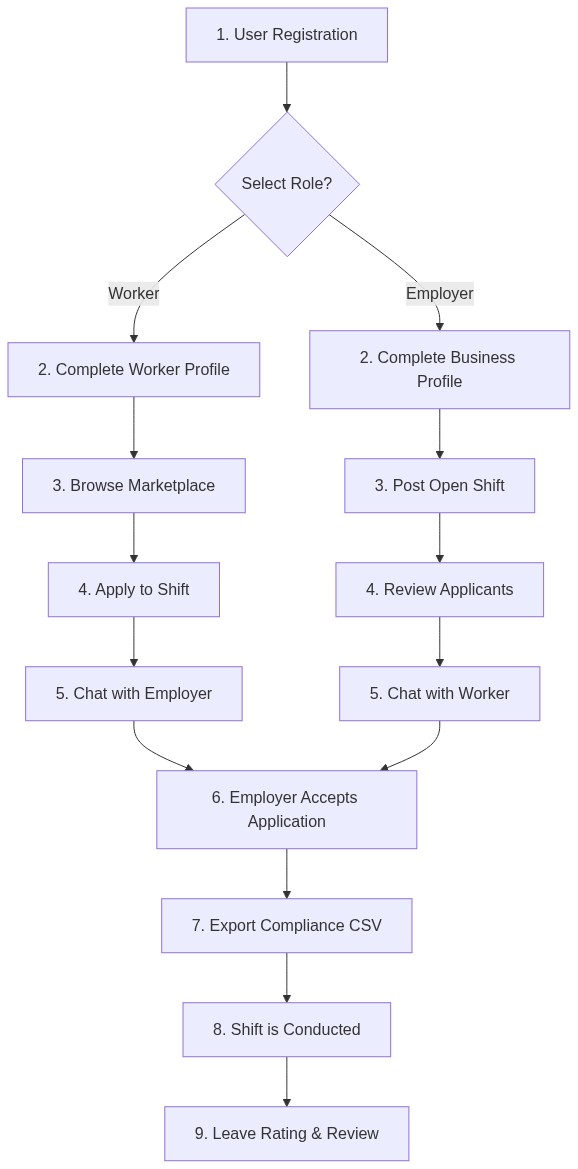
\includegraphics[width=\textwidth]{user_journey.png}
\caption{GigTim User Journey Flow}
\label{fig:user_journey}
\end{figure}

\end{document}
